% !TEX root = paper.tex
% !TEX encoding = UTF-8 Unicode
% -*- coding: UTF-8; -*-
% vim: set fenc=utf-8
% !TEX spellcheck = en-US
\section{Introduction}
\label{sec:intro}
\paragraph{Problem statement.}
%------------------------------%
%: see Figure~\ref{fig:intro}
\begin{figure}[b!]%%[p!]
	\centering{	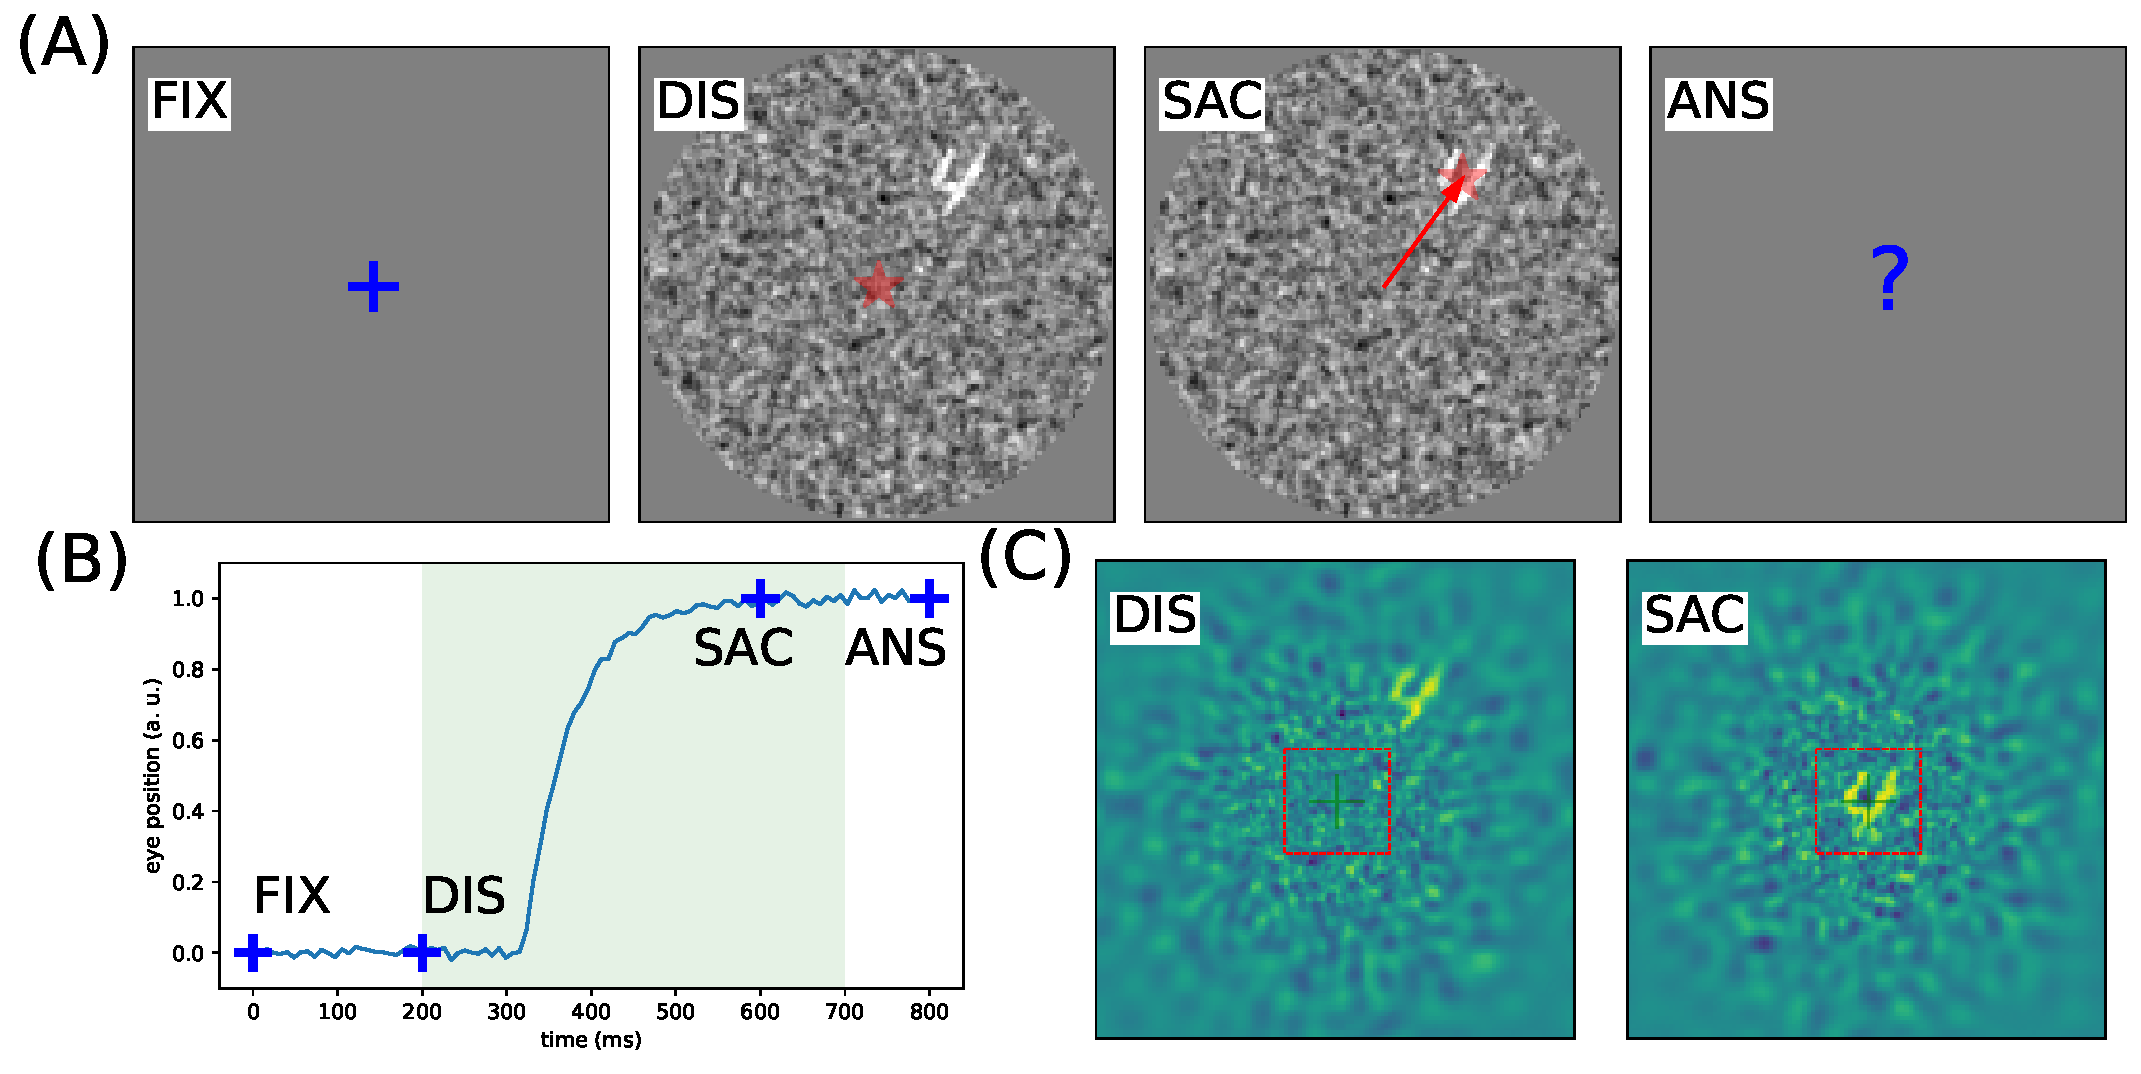
\includegraphics[width=\linewidth]{fig_intro}} %
	\caption{%
		{\bf Problem setting}: In generic, ecological settings, the visual system faces a tricky problem when searching for one target (from a class of targets) in a cluttered environment. It is synthesized in the following experiment: %
		\A After a fixation period \FIX\ of $200~\ms$, an observer is presented with a luminous display \DIS\ showing a single target from a known class (here digits) and at a random position. The display is presented for a short period of $500~\ms$ (light shaded area in B), that is enough to perform at most one saccade (here, successful) on the potential target \SAC . Finally, the observer has to identify the digit by a keypress \ANS . %
		\B Prototypical trace of a saccadic eye movement to the target position. In particular, we show the fixation window \FIX\ and the window during which a saccade is possible (green shaded area). %
		\C Simulated reconstruction of the visual information from the (interoceptive) retinotopic map at the onset of the display \DIS\ and after a saccade \SAC , the dashed red box indicates the visual area of the ``what'' pathway. In contrast to an exteroceptive representation (see A), this demonstrates that the position of the target has to be inferred from a degraded (sampled) image. In particular, the configuration of the display is such that by adding clutter and reducing the size of the digit, it may become necessary to perform a saccade to be able to identify the digit. The ``where'' pathway mediating the action has to infer the location of the target \emph{before seeing it}, that is before being able to actually be able to identify the target's category using the ``what'' pathway. %
		\label{fig:intro}}%
\end{figure}%
%%------------------------------%
The promise of artificial vision to identify objects in natural images is ever increasing. Image processing algorithms recently outreached the performance of human observers in specific image categorization tasks~\citep{He15}. Initially trained on energy greedy, high performance computers, they are now designed to work on more common hardware such as desktop computers with a decent GPU~\citep{Sandler18}. However, these algorithms are still outperformed by humans for simple tasks. Take for instance the case of an encounter with a friend in a crowded café. To catch the moment at which he will arrive, you need to visually search for his face despite all the remaining sensory clutter. To do so, you need to scan relevant parts of the visual scene with your gaze. Doing a saccade at these locations, you will be able to recognize your friend. The main difficulty of this task is to learn to categorize this particular object class given all possible spatial configurations and respective geometrical visual transformations. Such a visual experience can be formalized and simplified in a way reminiscent to classical psychophysical experiments: An observer is asked to classify digits (for instance as taken from the MNIST database) as they are shown on a computer display. However, these digits can be placed at random positions on the display, and visual clutter is added as a background to the image (see Figure~\ref{fig:intro}-A). This opens the possibility that the position of the object may be detected in the clutter without being identified in the first place  (see Figure~\ref{fig:intro}-C). This defines more precisely our problem: how can we localize an object in a large image while knowing \emph{a priori} its category but not its identity? This generic visual search problem is of broad interest in machine learning, computer vision and robotics, but also in neuroscience, as it speaks to the mechanisms underlying foveation and more generally to low-level attention mechanisms.

Inherent to this problem is the combinatorial explosion implied by an increasing number of parameters. State-of-the art classification architectures consequently contain many millions parameters while still handling relatively small images, with subsequent energy consumption increase. This introduces a trade-off between efficiency (fast enough to detect visual objects in a glance in autonomous driving as well as being able to extend it to resource-constrained devices like mobile phones) and average accuracy. Globally, this performance is  still lower than that of humans. Indeed, the human visual system can perform such a feat both rapidly, --~in less than 100 ms~\citep{Kirchner06}~-- and at a low energy cost ($<5~W$). On top of that, it is mostly self-organized, robust to visual transforms or lighting conditions and can learn with a few examples. If many different anatomical features may explain this efficiency, a main difference lies in the fact that its sensor (the retina) combines a non homogeneous sampling of the world with the capacity to rapidly change its center of fixation. Indeed, on the one hand, the retina is composed of two separate systems: a central, high definition fovea (a disk of about 6 degrees of diameter in visual angle around the center of gaze) and a large, lower definition peripheral area. On the other hand, the retina is attached on the back of the eye which is capable of low latency, high speed eye movements.  In particular, saccades allow for efficient changes of the position of the center of gaze: they take about $200~\ms$ to initiate, last about $200~\ms$ and usually reach a maximum velocity of approx 600 degrees per second. This behavior is prevalent during our lifetime (about a saccade every 2-3 seconds, that is, almost a billion saccade in a lifetime).  The interplay of those two features allows human observers to engage in an integrated action perception loop which sequentially scans and analyses the different parts of the image.
%It is one type of active inference~\citep{Friston12} (see below) and we will envision herein how to incorporate it to classical computer vision schemes.
% (1 / 2.5 * 3600 * 24 * 365 * 75 = 946080000.0 ~= .95e9) X (wakeful + REM = .66)
%
\paragraph{State of the art.}


To take advantage of this visuomotor behavior, it is of particular importance to understand both its computational and neurophysiological principles. First, the joint problem of target localization and identification is a classical problem of visual search in computer vision. It is very general and may address apparently simple questions such as ``find the green bottle on the table''. 
When restricted to a mere ``feature search''~\citep{Treisman80}, many solutions are proposed. Notably, recent advances in deep-learning have provided  efficient models such as faster-RCNN~\citep{Ren17} or YOLO~\citep{Redmon15}. This last implementation is particularly interesting for our sake as it predicts in the image the probability of proposed bounding boxes around the visual object. While rapid, the number of boxes greatly increases with image size and necessitates dedicated hardware. 
When limited to a few objects of interest in the image, this strategy amounts to a classical problem in neuroscience, that is, the transformation of a luminous image into a saliency map~\citep{Itti01}, essential to understand and predict saccades, but also to serve as phenomenological models of attention. The saliency approach was recently extended using deep learning  to estimate saliency maps over large databases of natural images~\citep{Kummerer16}. While these methods are efficient at predicting the probability of fixation, they miss an essential point in the action perception loop: they operate on the full image while the retina operates on the non-uniform, foveated sampling of visual space (see Figure~\ref{fig:intro}-B). Herein, we believe that this fact is an essential factor to reproduce and understand this active vision process.

In contrast to phenomenological (or ``bottom-up'') approaches, models of active vision~\citep{Najemnik05,Butko2010infomax,Friston12} provide the ground principles of saccadic exploration. They assume the existence of a generative model from which both the target position and category can be inferred through active sampling. This comes from the constraint that the visual sensor is foveated but can generate a saccade. 
Several studies are relevant to our endeavor. First, one can consider optimal strategies to solve the problem of the visual search of a target~\citep{Najemnik05}. In a setting similar to that presented in Figure~\ref{fig:intro}-A, where the target is an oriented edge and the background is defined as pink noise, authors show first that a Bayesian ideal observer comes out with an optimal strategy, and second that human observers are close to that optimal performance. Though predicting a sequence of saccades in a perception action loop, this model is limited by the simplicity of the display (elementary edges added on stationary noise, a finite number of locations on a discrete grid) and by the abstract level of modeling. Despite these (inevitable) simplifications, this study could successfully predict some key characteristics of visual scanning such as the trade-off between memory content and rapidity.

%Looking more closely at neurophysiology, t
The study of~\citep{Samonds18} allows to go further in understanding the interplay between saccadic behavior and the statistics of the input. In this study, authors were able to manipulate the size of the saccades by monitoring key properties of the presented (natural) images. For instance, smaller images generate smaller saccades. Interestingly, they also predicted the size of saccades for different species, including mice which lack a foveal region, from the size of visual receptive fields. One key prediction of this study which is relevant for our problem is the fact that saccades seem optimal to \emph{a priori} decorrelate the visual input, that is, to minimize redundancy in the sequence of generated saccades, knowing the statistics of the visual inputs.

A further modeling perspective is provided by~\citep{Friston12}. In this setup, a full description of the visual world is used as a generative process. %, here a face model made of independent components: mouth, nose, eyes, etc... An agent is completely described by giving the generative model governing the dynamics of its internal beliefs and is interacting with this image by scanning it through a foveated sensor, just as described in Figure~\ref{fig:intro}. 
Equipping the agent with the ability to actively sample the visual world %enables to explore the idea that actions (saccadic eye movements) are 
allows to interpret saccades as optimal experiments, by which the agent seeks to confirm predictive models of the (hidden) world. One key ingredient to this process is the (internal) representation of counterfactual predictions, that is the probable consequences of possible hypothesis as they would be realized into actions (here, saccades).
%Such a model constitutes 
Simulations of such an active inference scheme~\citep{Mirza18} 
%and simulations of the resulting optimization 
reproduce sequential eye movements that fit well with empirical data. %Compared to~\citet{Najemnik05}, 
Saccades %are not the output of a value-based cost function, but 
are here a consequence of an active seek for the agent to minimize the uncertainty about his beliefs, knowing his priors on the generative model of the visual world. %Such an approach applies well to our setting.
%, as described in Figure~\ref{fig:intro}. 
\if 1\ICANN
\else

\fi
%An interesting perspective is given with previous modeling of such foveated sensors. 
Finally, the non-uniform sampling of visual space is usually modeled as a log-polar conformal mapping~\citep{Traver10} which has a long history in computer vision and robotics. A first property of this mapping is the separation between the foveal and the peripheral areas as we defined above. This transformation has also other notable properties, such as the correspondence by way of translations in the radial and angular directions to respectively rotations and scalings in the visual domain. However, this sensor is to our knowledge most often not coupled to an action
\if 1\ICANN
\else
 (but see~\citep{ref_needed)}\fi. 

\paragraph{Outline.}
%The goal of this work is thus to emulate a model of active vision which is able to infer the position of a visual target independently from its category.
Stemming from the active vision general principles, our aim is to produce a principled model that may both explain the essential features of human vision and provide ways toward efficient computer implementations. 
\emph{We also aim at reunifying the fragmentation of the many different approaches respective to their fields (Machine learning, neuroscience, robotics), and envisage an integrated computational model of foveated active vision.}


%However, inverting a generative model over a large (one-step ahead) hypothesis space of all possible saccades is computationally-intensive. % (think for instance of face category as a very large categorical space over a large visual transformation space) with no obvious neurophysiological counterpart.  (see Figure~\ref{fig:intro}-C)
%Although we similarly include a generative process of the visual world,
In particular, complex combinatorial inferences are here replaced by separate pathways, i.e. the spatial (``where'') and categorical (``what'') pathways, whose knowledge is combined to infer optimal eye displacement and subsequent identification.    
%as conatining {\bf (containing??)} images of a handwritten random digit (drawn from the MNIST database) at a random position and embedded in a cluttered noise . 
In addition,  the agent is equipped with a foveated sensor, %and with the ability to actively scan the visual image as defined by a generative (internal) modelWe will use this constraint as an asset to 
which also contributes to minimizing the overall computational cost of finding a target. Taking such priors, we optimize the behavior of this agent and explore its key properties.
To that aim, this paper is organized as follows.

After this introduction, we define the methods in section~\ref{sec:methods}. First we  define notations, variables and equations for the generative process governing the experiment and the generative model for the active vision agent. In particular, we  derive our method to simplify the learning of an optimal agent given these definitions. In section~\ref{sec:results}, we  then show results of numerical simulations of this agent. We  first demonstrate some applications of this framework to different levels of complexity of the problem. This  allows us to derive some limits of this agent and, as in~\citep{Najemnik05}, we  draw some analogies with biologically observed eye movements. Finally, in section~\ref{sec:discussion}, we  summarize these results in comparison with other similar schemes. We  conclude by showing the relative advantages of using this active inference approach.
